\section{Domains with 0-Cost Actions}
\label{sec:zerocost-domains}
%% best to put openstacks here, considering the connection to the
%% previous section
\pddl{Openstacks}  is a cost
minimization domain introduced in IPC-2006, where the objective is to 
minimize the number of stacks used.
One characteristic of \pddl{Openstacks} is the presence of many  actions which have zero cost because they do not increase the number of stacks. These 0-cost actions create the problem depicted in \refig{fig:plateau-1}.
% Since 0-cost actions corresponds to 0-cost search edges.
% If such actions are present, the neighbors of the goal nodes could be surrounded by the 0-cost edges.
Since 0-cost actions (edges) allow ``free'' transitions between many neighboring nodes,
the number of neighboring nodes sharing the same $h$ also becomes quite large.
This creates huge plateaus that share the same $h$-value, and the standard $h$-based tie-breaking criterion can not provide informative guidance for search within a plateau.\todo*{why mention $f=f^*$ specifically here, instead of ``final plateau'' (f*,0) or just in general all plateaus?}
Since the $g$-values of the nodes in these plateaus are all identical, these plateaus are an instance of $g$-value plateaus, which are known to increase the difficulty of search \cite{benton2010g}.

\begin{figure}[htbp]
  \centering
  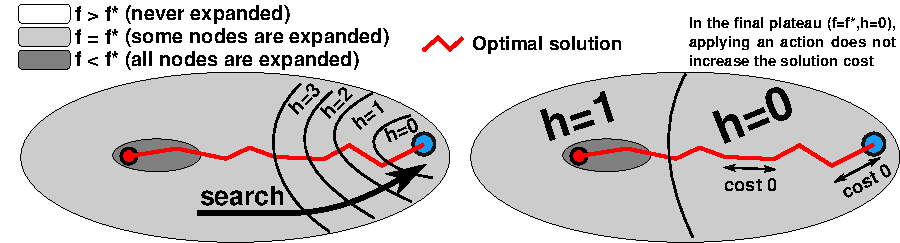
\includegraphics{img/astar/plateau-1.pdf}
 \caption{Search space of \astar and its contour according to admissible heuristic $h$. (\textbf{Right}) In domains with only positive-cost actions, $h$-based tie-breaking provides meaningful guidance. (\textbf{Left}) In domains with 0-cost actions, applying an action may not increase the cost of the path and the region with $h=0$ could be quite large. With the same mechanism, other heuristic plateaus (e.g. $h=1$) also become larger. Thus, $h$-based tie-breaking fails to provide meaningful guidance in this space.
  }
 \label{fig:plateau-1}
\end{figure}


%% safe to remove these explanation.
% According to \cite{richter2010lama}, \textbf{??????}
% %Richter talks about the failures on openstacks starting around p.167
% \lmcut \cite{Helmert2009} fails to find a good cost
% partitioning with non-zero values, 
% % A detailed discussion of Openstacks domain and poor performance of landmarks is in \cite{richter10lama}, p.167-169.
% and most edges in the abstraction
% space of M\&S \cite{helmert2007flexible} have zero costs.

% XXX I'm commenting out the paragraphs below because:
% (1) A review of heuristic functions for domain-independent learning is not really
% necessary for this AAAI submission. 
% (2) It's better if this paper is not so strongly associated with the ICAPS community only -- this work applies in general to search with A*, and is not strongly tied to almost-perfect heuristics, lmcut, m&s, etc.

Although most traditional benchmark problems in the planning community and the combinatorial search community do not have 0-cost actions,
we argue that such domains are of an important class of models for cost-minimization problems, i.e.,
assigning 0-costs makes sense from a practical, modeling perspective.
For example, consider the \pddl{driverlog} domain, where the task is to move packages between locations using trucks.
The IPC version of this domain assigns unit costs to all actions. Thus, cost-optimal planning on this domain seeks to minimize the number of steps in the plan.
However, another natural objective function would be the one which minimizes the amount of fuel spent by driving the trucks,
assigning cost 0 to all actions except \pddl{drive-truck} -- we believe that for cost-optimal planning, this is at least as natural as the current IPC model of \pddl{driverlog} in which all actions are of unit cost.

% While I agree with the point you're trying to make,
% There is an ugly issue when arguing that current models try to  optimize plan-execution time (i.e., makespan), 
% which is that if we really cared about makespan optimality, we would consider parallel execution of actions whenever possible.
% however, sequential classical planners do not handle parallel actions at all  (recall ACP).
% so arguing this path can only lead to trouble.. Let's try a safer line of argument.
%% For runtime minimization,
%% nonzero positive costs are reasonable because
%% every actions are supposed to consume a fraction of time.
%% However, such formulation is not suitable for general optimization
%% problems.  For example, when you try to minimize the energy consumption
%% by the elevators in \pddl{Elevators} domain, many actions would have 0-cost
%% --- it does not consume electricity for either boarding or leaving the
%% passenger, or moving the elevator down.
%% % 
%% From the practical point of
%% view, cost minimization domains would have wider interest compared to
%% the simple runtime minimization.
%% Also, as shown previously, such domains pose a
%% difficulty to the current heuristic planners due to their large plateaus.

Similarly, for many practical applications, a natural objective is to
optimize the usage of one key consumable resource, e.g., fuel/energy
minimization.  In fact, two of the IPC domains, \pddl{Openstacks} and
\pddl{Cybersec}, which were shown to be difficult for standard tie-breaking
methods in the previous section, both contain many 0-cost actions
and are based on industrial applications: %no textbf here because both \pddl{Cybersec} and \pddl{Openstacks} are highly simplified models, let's not exaggerate their importance
\pddl{Openstacks} models
production planning \cite{fink1999applications} and \pddl{Cybersec}
models Behavioral Adversary Modeling System \cite[minimizing decryption,
data transfer, etc.]{boddy2005course}.

Therefore, %In order to create a benchmark set that better addresses practical interest, % don't add new claims that make judgements about previous work (benchmark sets) 
in this paper, we modified various standard domains
into cost minimization domains with many 0-cost actions.
Specifically, each of our ``Zerocost domains'' is a standard domain which has been modified so that all action schema are assigned
cost 0 except for a few (usually one) action schema which consumes some key resource.
The suffixes in the names of these domains indicate the actions with non-zero costs, 
%e.g., \pddl{elevator-up} is a modified elevator
%domain where the \pddl{up} action is assigned non-zero cost (because
%elevators are considered to consume energy only when going \pddl{up}), 
% I believe elevators use some energy when going down as well, so let's not highlight this example.
e.g., \pddl{logistics-fuel} is a modified logistics domain where only actions which consume fuel have non-zero cost.
Most of the transportation-type domains are modified to optimize 
energy usage (\pddl{logistics-fuel}, \pddl{elevator-up} etc.), and  assembly-type domains are modified to minimize resource usage
%% \pddl{floortile-ink} is not shown, so better not to mention it
(\pddl{Woodworking-cut} minimizes wood usage, etc.).
When no action makes sense from the practical point of view, we chose an action schema arbitrarily (e.g. \pddl{mprime-succumb}).
We did not
include domains which have only a single action schema, or which already had many 0-cost actions.

The new set of 28 \emph{Zerocost domains} are:
\pddl{airport-fuel} (20 instances), \pddl{blocks-stack} (20), \pddl{depot-fuel} (22), \pddl{driverlog-fuel} (20),
\pddl{elevators-up} (20), \pddl{floortile-ink} (20), \pddl{freecell-move} (20), \pddl{grid-fuel} (5),
\pddl{gripper-move} (20), \pddl{hiking-fuel} (20), \pddl{logistics00-fuel} (28), \pddl{miconic-up} (30),
\pddl{mprime-succumb} (35), \pddl{mystery-feast} (20), \pddl{nomystery-fuel} (20),
\pddl{parking-movecc} (20), \pddl{pathways-fuel} (30), \pddl{pipesnt-pushstart} (20),
\pddl{pipesworld-pushend} (20), \pddl{psr-small-open} (20), \pddl{rovers-fuel} (40),
\pddl{scanalyzer-analyze} (20), \pddl{sokoban-pushgoal} (20), \pddl{storage-lift} (20),
\pddl{tidybot-motion} (20), \pddl{tpp-fuel} (30), \pddl{woodworking-cut} (20),
\pddl{zenotravel-fuel} (20).

While the action costs in the PDDL \emph{domain} definitions are modified,
we did not modify the PDDL \emph{problem} definitions.
Although some domains (specifically, \pddl{blocks}, \pddl{freecell}, \pddl{pipesworld-notankage}, \pddl{miconic}) have fewer instances than the original domain does,
their problem definitions are the evenly sampled subset of the original set of instances.
% \pddl{blocks} original 35 vs 20, \pddl{freecell} 80 vs 20, pipesnt 50 vs 20, \pddl{miconic} 150 vs 30
For example, the original \pddl{miconic} domain has 150 instances, while our version has 30 instances.
These 30 instances are selected evenly from the original set of instances, by picking instances p05, p10, ... p150.
% 
The reason for reducing the number of instances is to avoid the problem of the overall coverage sums being skewed by the domains with a larger number of instances.
Thus, we did not modify the problem definitions at all, and only modified the action costs in the domain definitions.

\subsection{Difference in Problem Characteristics between IPC and Zerocost Domains}

Domains containing 0-cost operators are known to be difficult for traditional planners \cite{thayer2009using,cushing2010cost,wilt2011cost,thayer2011bounded,richter2011lama}.
\citeauthor{cushing2010cost} \citeyear{cushing2010cost} and \citeauthor{wilt2011cost} \citeyear{wilt2011cost} noted that a large ratio between maximum and minimum operator costs can pose a challenge to existing planners. They both addressed this using plan-length heuristics instead of plan-cost heuristics, which sacrifice the optimality of the solution. In contrast, we investigate methods for handling 0-cost operators within the framework of admissible search. In \refsec{sec:distance-to-go}, we show how  plan length heuristics can be incorporated into admissible search.
%While \citeauthor{cushing2010cost} \citeyear{cushing2010cost} and \cite{wilt2010cost} \citeyear{wilt2011cost} also analyze the cause of difficulties,  % if we don't say the causes they determined are, then no need to say they analyzed
In a parameterized complexity analysis of planning domains,
\citeauthor{aghighi2015} \citeyear{aghighi2015,aghighi2016} % fully complemented the full theory behind this, % don't casually use strong terms like ``fully''
showed % can't extrapolate too strongly from problem class complexity results to specific instances 
that domains with 0-cost operators comprise a complexity class that is harder (para-\textbf{NP}-hard) than the domains with strictly positive-cost operators (\textbf{W}[2] complete), 
indicating the inherent difficulty of optimally solving planning problems with 0-cost actions.

% Previous empirical work on domains with 0-cost operators has focused on relatively few domains: Grid Path Planning, Blastlands, Zenotravel \cite{thayer2009using}, Zenotravel \cite{cushing2010cost}, Sliding Puzzle, Pancake Puzzle, Sliding Puzzle \cite{wilt2011cost}, Dock Robot, Vacuum World, Robot Navigation, Sliding Puzzle\cite{thayer2011bounded}.

%To our knowledge, an empirical study on such differences over a wide range of IPC domains is missing in the literature,
%Thus it is expected that there would be significant performance differences when a domain independent planner solves the original IPC instances and our Zerocost instances.

% M\&S comparison can be removed even from the appendix.
% The result is not essential. Furthermore,
% these numbers can be extracted from the other tables.
Therefore we experimentally evaluate whether our new set of Zerocost benchmarks based on standard IPC domains pose a new challenge for
standard tie-breaking strategies. Results using the \lmcut
 % and \mands
heuristic are shown in \reftbl{tbl:lmcut-zerocost-std}%  and
% \reftbl{tbl:mands-zerocost-std} (Appendix), respectively
. In each table,
the left-hand side shows the results in the original domains and the right-hand side
shows the results for the corresponding Zerocost domains.
%We excluded domains whose
%number of instances in the standard domain differs from the number of instances in the 0-cost version. % this is noted in the table caption

%For both \lmcut and \mands heuristics,
We observed a significant
performance difference between the original IPC domains and the Zerocost
domains.
%With \lmcut, t
The coverage in Zerocost domains
was lower in 11 domains while more instances were solved
in 5 domains.
%With \mands, the coverage in Zerocost domains was lower in 10 domains while
%more instances were solved in 3 domains.
\todo*{Can we consolidate the lmcut table mands table comparing the 0-cost vs standard domains?  Doesn't seem important enough for 2 tables --- not critical}
The coverage increase in some domains is not surprising, considering that 0-cost actions also make some suboptimal paths into cost-optimal paths. However, the coverage decreased overall, confirming the difficulty of these domains.

\refig{fig:plateau-zerocost} plots the size of the final plateau of the
Zerocost instances, with \lmcut heuristics and $h$ tie-breaking. In this plot,
each point shows the total number of nodes in $\plateau{f^*,0}$ vs the
total number of nodes with $f\leq f^*$. Compared to \refig{fig:plateau},
most Zerocost instances have larger plateaus even with the help of
$h$ tie-breaking.  Thus, in these cost-minimization problems, the search
strategy within plateaus, i.e., tie-breaking, becomes even more critical
in determining search performance.

% summary data ?

\begin{table}[htbp]
 \centering
 \setlength{\tabcolsep}{0.2em}
\begin{center}
\begin{tabular}{|lc|ccr|}
 & solved & solved & (difference) & \\
depot(22) & 6 & 6 &  & depot-fuel(22)\\
driverlog(20) & 13 & 8 & (-5) & driverlog-fuel(20)\\
elevators-opt11(20) & 15 & 7 & (-8) & elevators-up(20)\\
floortile-opt11(20) & 6 & 8 & (+2) & floortile-ink(20)\\
grid(5) & 1 & 1 &  & grid-fuel(5)\\
gripper(20) & 6 & 7 & (+1) & gripper-move(20)\\
logistics00(28) & 20 & 16 & (-4) & logistics00-fuel(28)\\
mprime(35) & 21 & 15 & (-6) & mprime-succumb(35)\\
nomystery-opt11(20) & 14 & 10 & (-4) & nomystery-fuel(20)\\
parking-opt11(20) & 1 & 0 & (-1) & parking-movecc(20)\\
pathways(30) & 5 & 5 &  & pathways-fuel(30)\\
rovers(40) & 7 & 8 & (+1) & rovers-fuel(40)\\
scanalyzer-opt11(20) & 10 & 9 & (-1) & scanalyzer-analyze(20)\\
sokoban-opt11(20) & 19 & 18 & (-1) & sokoban-pushgoal(20)\\
storage(30) & 14 & 4 & (-10) & storage-lift(20)\\
tidybot-opt11(20) & 12 & 16 & (+4) & tidybot-motion(20)\\
tpp(30) & 6 & 8 & (+2) & tpp-fuel(30)\\
woodworking-opt11(20) & 10 & 5 & (-5) & woodworking-cut(20)\\
zenotravel(20) & 11 & 7 & (-4) & zenotravel-fuel(20)\\
\end{tabular}
\end{center}

 \caption{
 Assessment of the relative difficulty of Zerocost domains vs. their corresponding standard domains, for the standard $[f,h,\fifo]$ strategy.
 Coverage comparison (the number of instances solved) 
 between the original IPC domains and the modified Zerocost domains are shown, 
 using the same planner configuration and experimental setting (5min, 4GB, \lmcut heuristics).
 This table does not include domains where the total number of instances
 in the Zerocost domain  and the original domain differ. 
 }
 \label{tbl:lmcut-zerocost-std}
\end{table}

\begin{figure}[htbp]
  \centering
  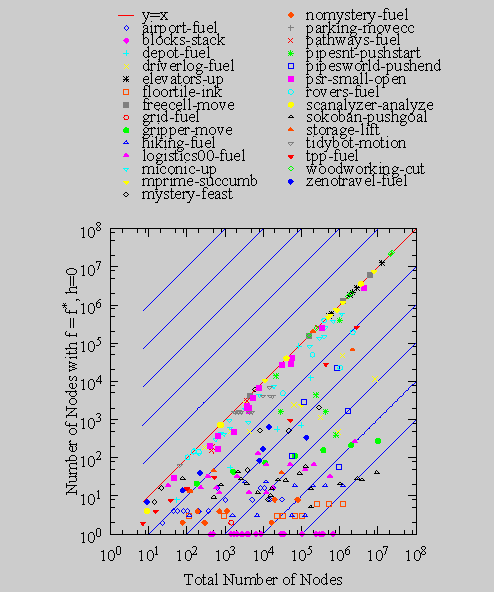
\includegraphics{tables/aaai16-frontier/zerocost/lmcut_frontier-front.pdf}
  \caption{
 The number of nodes in $\plateau{f^*, 0}$ (y-axis), which form
  the final plateau under $h$-based tie-breaking, compared to
 the total number of nodes in the search space (x-axis) with
 $f\leq f^*$ on 620 instances in our \emph{Zerocost domains}.
 The final plateaus tends to account for a larger portion of the
 entire search space compared to \refig{fig:plateau}.
 These statistics are obtained by running a modified Fast Downward with
 \lmcut which continues searching after the solution is found
 until expanding all nodes with cost $f=f^*$.
 }
 \label{fig:plateau-zerocost}
\end{figure}

\subsection{Discussion on Zerocost Domains}

Trivially, changing the edge costs does not make a finite graph infinite.
Thus, 
the search graph of the Zerocost versions of the instances remains finite
if the search graph of the original instance is finite,
which is the case with domain-independent planning under STRIPS semantics.
Since \astar is complete on a finite graph regardless of the tie-breaking strategy,
Zerocost domains do not affect the completeness of the search.

Note that the difficulty posed by these domains sometimes \emph{cannot}
be tackled by improving the heuristic estimates, or reducing the
underestimation of an admissible heuristic function.  Due to the
existence of 0-cost edges, some non-goal neighbors of a goal node 
% admissibly 
have $h^*=0$. For those nodes,
there is clearly no room for improving the heuristic estimate; Any positive
value causes the heuristics to be inadmissible.
% this quote is stylistically inappropropriate; also, should not add sentences that can be interpreted as new claim about relationship to  previous work that need to be reviewed.
%Thus it would be safe to say that this is another instance where
%``further improvements in run-time require
%changes to other parts of the search algorithm than the heuristic estimator''
% \cite{helmert2008good}.

One approach to improving the search performance in such plateaus
produced by 0-cost edges is to perform an efficient
\emph{knowledge-free} search within plateau; It may reuse the effort
that is already spent to guide the search but without requiring 
additional effort to compute multiple heuristics.
In the next section, we propose and evaluate an implementation of
such a technique. It turns out that introducing a notion of \emph{depth} within a plateau can have
a significant impact on the performance of knowledge-free search, and can also 
provide a good  understanding of the behavior of standard tie-breaking strategies.

